\documentclass[10pt,conference,compsocconf]{IEEEtran}

%\usepackage{times}
%\usepackage{balance}
\usepackage{url}
\usepackage{graphicx}
\usepackage{amsmath}
\usepackage{amsfonts}
\usepackage{caption}

\begin{document}
\title{An Ensemble of stacked models for Collaborative Filtering}

\author{
  Andrea Rinaldi, Simon Haefeli, Giuseppe Russo, Gianni Perlini\\
  Kaggle Group Name: Team Name \\
  Department of Computer Science, ETH Zurich, Switzerland
}

\maketitle

\begin{abstract}

Recommender Systems are used by tech companies such as Netflix and Amazon to perform targeted advertising. A common technique used to design such systems is Collaborative Filtering (CF), which works by analysing data on users' information such as, for example, movies' ratings and items preferences in general. In this project we implement 7 different models for CF and then combine them using ensemble learning to further improve the results of our predictions. We use Singular Value Decomposition (SVD) and Matrix Factorization with Stochastic Gradient Descent (MF with SGD) as our baselines and compare our improvements over them. Some of the methods we used includes Bayesian Probabilistic Matrix Factorization (BPMF) and Non-parametric Principal Component Analysis (NPCA). The results are obtained using the provided dataset from Kaggle.

\end{abstract}

\section{Introduction}
\label{int}

Recommender systems are used in multiple situations in today's Internet, mainly for commercial purposes. They can be found in e-commerce applications to recommend items to purchase, or in on-line video streaming to give advice on which movie to watch next. An example of companies using these systems are Netflix and Amazon. These types of companies are confronted with millions of users and items which gives rise to the need of having a recommender system which is both reliable and efficient, while dealing with an increasing amount of data. A common technique to design recommender systems is collaborative filtering. This technique uses users' past behaviour (preferences, ratings, ...) to make predictions about what they could be interested in.\\
Common approaches in collaborative filtering are so called memory based techniques such as user-based or item-based, that measure the similarity between a given user and the other users, respecitvely a given item and the other ones, to predict the missing ratings. Other types of CF methods are model-based techniques such as PCA and SVD, and often use a matrix factorization approach to predict the missing entries. These different methods have widely been studied during the past years and all come with their strengths and limitations. To overcome such weaknesses, a hybrid approach is often used in order to combine multiple models. This allows the recommender system to benefit from the advantages of different techniques while minimizing their individual limitations.\\
In this paper we implement 7 different models which separately predict the missing entries, and then combine the predictions from each model using Ridge Regression or \textbf{M}ulti \textbf{L}ayer \textbf{P}erceptron (MLP).\\
Our paper is structured as follows: in \emph{Section \ref{mam}} we present the mathematical description of the models and give some details about their implementations. In \emph{Section \ref{res}} we show the results obtained by performing prediction with our approach, and we discuss these results in \emph{Section \ref{disc}}. We conclude our paper in \emph{Section \ref{conc}}.

\section{Models and Methods}
\label{mam}

In this section we describe the problem we are tackling as well as the models we used to solve it.

\subsection{Problem Description}

We are given a dataset of 10000 users and 1000 items with 11.76\% of rating density. Our goal is to predict the missing rating $r_{ij}$ given by user $i$ to the $j$-th movie. All ratings are integer numbers between 1 and 5. The evaluation of the predictions is done according to the \textbf{R}oot \textbf{M}ean \textbf{S}quared \textbf{E}rror (RMSE), which is defined as:

$$
RMSE = \sqrt{\frac{1}{\vert N \vert} \sum_{(i,j)\in N} (r_{ij} - \hat{r}_{ij}})^2
$$

\noindent where $r_{ij}$ is the true rating, $\hat{r}_{ij}$ is the predicted one and $N$ is the set of user-movie pairs that we want to evaluate.

\subsection{Models Description}

%TODO add implementations' params

\begin{description}

\item[\emph{Item-based with Pearson}]\ \\
This method uses similarity between items' ratings to recommend items to the target user. As a measure of similarity we use Pearson's correlation, which is defined \cite{Sarwar:2001:ICF:371920.372071} as follows :
$$
sim_p(i, j) = \frac{\sum_{u \in U} (r_{i,u} - \bar{r_i})(r_{j,u} - \bar{r_j})}{\sqrt{\sum_{u \in U} (r_{i,u} - \bar{r_i})^2}	\sqrt{\sum_{u \in U} (r_{j,u} - \bar{r_j})^2}}
$$

where $U$ represents the set of users that rated both item $i$ and $j$, and $\bar{r_i}$ (resp. $\bar{r_j}$) is the average rating of item $i$ (resp. $j$). The result is a value comprised in the interval $[-1;1]$, where +1 indicates maximum similarity between the items while a value of 0 means that the two ratings seems to be independent. \\
Once we have the similarity coefficients, we compute the prediction on an item $i$ for user $u$ by computing the sum of the ratings given by the user on the items similar to $i$. Each rating is weighted by the corresponding similarity $s_{i,j}$ between items $i$ and $j$. Formally:

$$
\hat{r_{i,u}} = \frac{\sum_{j \in I_i} (sim_p(i, j) \ast r_{u,j} )}{\sum_{j \in I_i} \vert sim_p(i, j) \vert}
$$ 

where $I_i$ represents the set of items similar to item $i$.
\item[\emph{Regularized SVD}]\ \\
This method combines SVD with regularized SGD to make predictions on users' ratings. The data matrix is first decomposed into two matrices $\textbf{U} = \left[ u_i \right]$ and $\textbf{V} = \left[ v_j \right]$ representing the user and item latent feature matrices where $u_i,v_j \in \mathbb{R}^k$. The predicted rating is then given by $\hat{r}_{ij} = u_i^Tv_j + p_i + q_j$ where $p_i$ and $q_j$ are the biases of user $i$ and item $j$ respectively. We then use SGD with regularization \cite{paterek} to estimate $u$ and $v$ as follows :

$$
\begin{aligned}
& e_{ij} = r_{ij} - \hat{r}_{ij} \\
& u_{ik} += \eta \ast (e_{ij}v_{jk} - \lambda u_{ik}) \\
& v_{jk} += \eta \ast (e_{ij}u_{ik} - \lambda v_{jk}) \\
& p_{i} += \eta  \ast (e_{ij} - \gamma (u_i + v_j - b)) \\
& q_{j} += \eta  \ast (e_{ij} - \gamma (u_i + v_j - b))
\end{aligned}
$$

\noindent where $e_{ij}$ is the error between the true rating $r_{ij}$ and the predicted one $\hat{r_{ij}}$, $\eta$ is the learning rate, $\lambda$ is the regularization term for $u$ and $v$, $\gamma$ is the regularizer for the biases and b is the global bias. After having tried different combinations for $\lambda$, $\gamma$ and the number of latent facators ($k$), we achieved the best score on the validation set with $k = 12$, $\lambda = 0.05$ and $\gamma = 0.15$. In the results, we will refer to this method as RSVD.
\item[\emph{Post-processing SVD with Kernel Ridge Regression}] \ \\
This method combines Ridge regression with the kernel trick to improve SVD  \cite{paterek}. To do that, the $u_{ik}$ weights are discarded and the $v_{jk}$ are used as predictors. Defining $y$ as the vector of movies rated by user $i$ and let $X$ be a matrix of observations - each row of $X$ is normalized vector of features of one movie $j$ rated by user $i$: $x_j = \frac{v_j}{\Vert v_j \Vert}$. The prediction of $y$ by ridge regression is given by	:

$$
\hat{y}_i = x_i^T(X^TX + \lambda I)^{-1}X^Ty
$$

\noindent Using an equivalent formulation involving Gram matrix $XX^T$ and the kernel trick, we get the following prediction:

$$
\hat{y}_i = K(x_i^T,X)(K(X,X) + \lambda I)^{-1}y
$$

\noindent where $K$ is, in our case, a Gaussian kernel defined as $K(x_i^T, x_j^T) = \exp(2(x_i^Tx_j-1))$ and $\lambda = .7$. In the results, we will refer to this method as Ridge SVD.
 
 
\item[\emph{K-means++}]\ \\
We implement an improved version of the vanilla k-means algorithm, performing an improved initialization algorithm for the cluster centroids. The intuition behind this approach is that spreading out the k initial cluster centers is a good thing: the first cluster center is chosen uniformly at random from the data points that are being clustered, after which each subsequent cluster center is chosen from the remaining data points with probability proportional to its squared distance from the point's closest existing cluster center. For this particular application (CF), the k-means algorithm is used to divide users into $K$ clusters $C_k$ and minimizing the intra-cluster variance, defined in \cite{paterek} as:

$$
\sum_{k=1}^K \sum_{i \in C_k} \Vert y_i - \mu_k \Vert^2 = \sum_{k=1}^K \sum_{i \in C_k} \sum_{j \in J_i} (y_{ij} - \mu_{kj})^2
$$

\noindent where $J_i$ is the set of movies rated by user $i$ and $\mu_{kj}$ is the prediction for rating of each user in $C_k$ given to movie $j$.

We performed the k-means algorithm for different numbers of clusters, from 4 to 24 with an inerval step of 2. Lastly, since the error in these configuarations decreases almost linearly, without a clearly noticeable "knee" in the error plot, we decided to use as predictions, the mean of the predictions across the aforementioned configurations.

\item[\emph{BPMF}] \ \\
This method aims at improving Probabilistic Matrix Factorization techniques by taking a Bayesian approach, and is described in \cite{BPMF}. In traditional probabilistic matrix factorization the user-specific and movie-specific latent feature matrices $U$ and $V$ are assumed to be Gaussian with mean 0 and covariance $\alpha^{-1} I$, where $\alpha$ is a precision factor.  
In BPMF, the conditional distribution over the observed ratings $R$ and the prior distributions over user-specific and movie-specific latent feature matrices $U$ and $V$ are assumed to be Gaussian with mean $\mu_{U}$ and covariance $\Lambda_{U}$, respectively $\mu_{V}$ and $\Lambda_{V}$, whereas the user and movie hyperparameters ($\Theta_{U}=\{\mu_{U},\Lambda_{U}\}, \Theta_{V}=\{\mu_{V},\Lambda_{V}\}$) are assumed to follow a Wishart-Gaussian or a gaussian distribution:
$$
\begin{aligned}
p(\Theta_{U} \vert \Theta_{0}) =  \mathcal{N}(\mu_{U} \vert \mu_{0}, (\beta_{0}\Lambda_{U})^{-1})\mathcal{W}(\Lambda_{U} \vert W_{0}, \nu_{0})
\end{aligned}
$$
and the prediction of rating $R_{ij}^*$ is obtained by marginalizing over the model parameters and hyperparameters:

$$
\begin{aligned}
p(R_{ij}^* \vert R, \Theta_0) =  \int\int p(R_{ij}^* \vert U_i,V_j)p(U,V \vert R, \Theta_U \Theta_V) \\
p(\Theta_U \Theta_V \vert \Theta_0)d \left\lbrace U,V \right\rbrace  d \left\lbrace \Theta_U, \Theta_V \right\rbrace
\end{aligned}
$$
\noindent However, this evaluation is intractable. The authors of the paper thus suggest to use an MCMC-based method to approximate the above integrals. In particular, they use the Gibbs sampling algorithm to implement BPMF as shown in \emph{Figure \ref{gibbs}}.

\begin{figure}[t!]
\centering
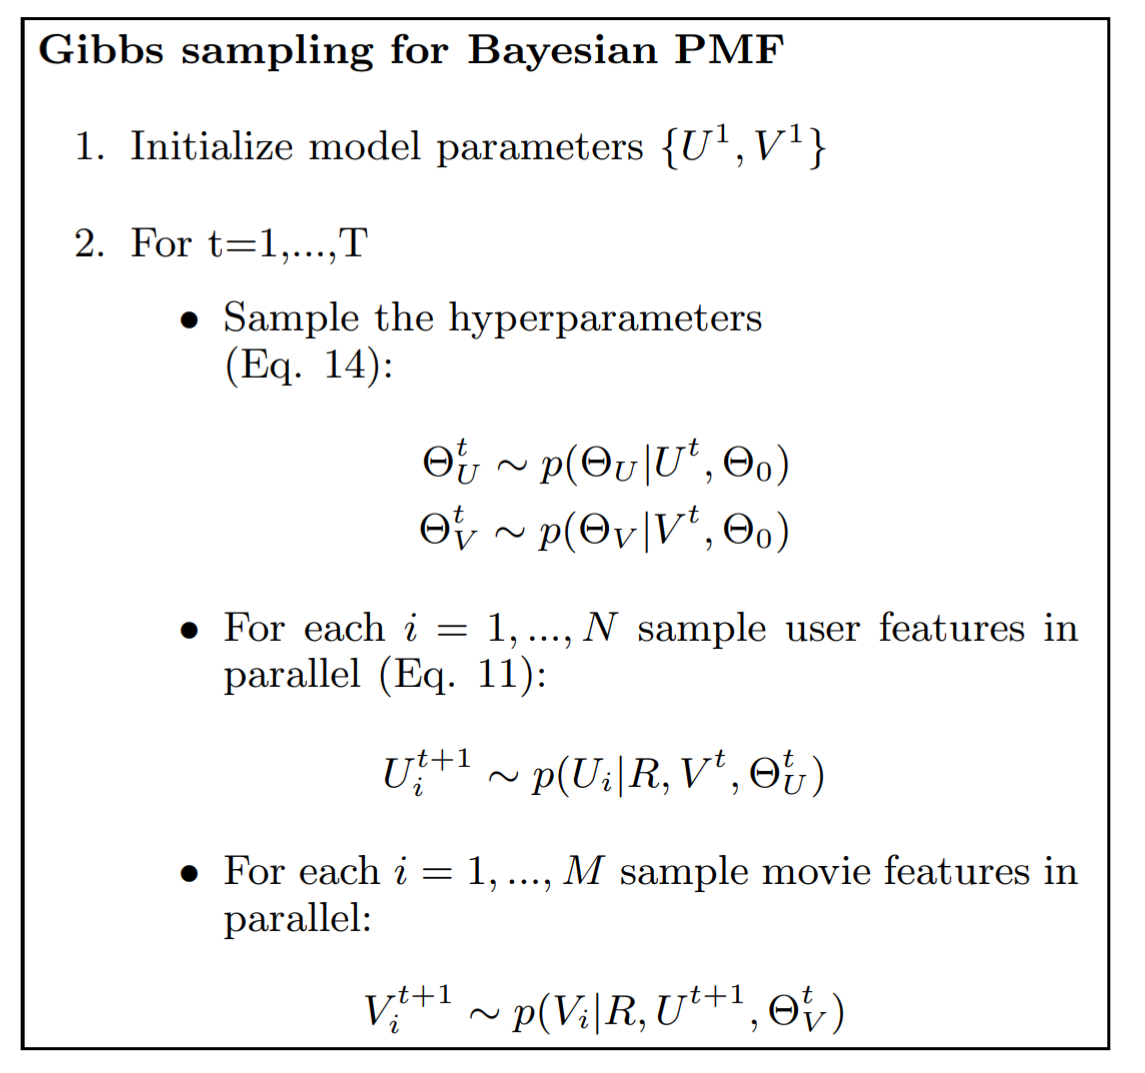
\includegraphics[scale=0.35]{gibbs.png}
\caption{Gibbs sampling algorithm as shown in \cite{BPMF}}
\label{gibbs}
\end{figure} 

\item[\emph{NPCA}] \ \\
NPCA is an extension of Probabilistic PCA which deals with infinitely many latent factors. We implemented the model following \cite{npca}. In this situation, working directly with the vector of latent factors $\textbf{u}$ and $\textbf{v}$ is intractable and the vector $\textbf{x}_i = \left[u_i^Tv_1, \dots , u_i^Tv_j, \dots , u_i^Tv_N \right] $ is used instead. The model then describes a latent process $X$ and an observational one $Y$ described by the following distribution:
$$
\int p(Y,X \vert K, \lambda)dX = \prod_{i=1}^M \mathcal{N}(y_{\mathbb{O}_i};0, K_{\mathbb{O}_i} + \lambda I)
$$

\noindent where Y is the user-item matrix, K and lambda some hyperparameters, and $\mathbb{O}_{i}$ the indices of the observed items for a given user $i$. This equation is maximized using an EM algorithm. The authors formalize a fast EM algorithm that avoids computing an NxN inverse matrix called Fast NPCA which is depicted in \emph{Figure \ref{emnpca}}.

\begin{figure}[t!]
\centering
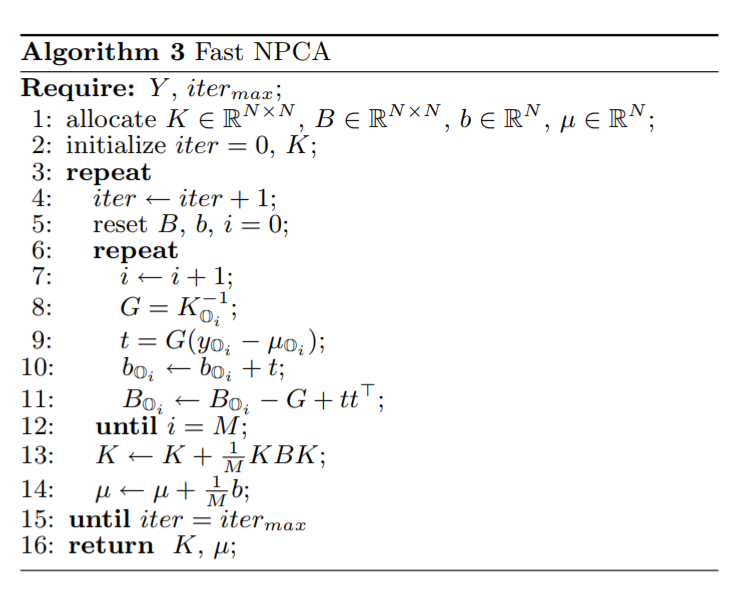
\includegraphics[scale=0.6]{emnpca.png}
\caption{Fast NPCA EM algorithm as shown in \cite{npca}}
\label{emnpca}
\end{figure} 

\item[Autoencoder] \ \\
An autoencoder provides a method to learn a non-linear mapping from $\mathbb{R}^{m}$ to $\mathbb{R}^{m}$. As shown in \cite{autorec}, this neural network can be adapted to the problem of collaborative filtering determined by a user-item rating matrx $M \times N$, by using each partially observed item vector $I_{i} \in {R}^{m} , i \in \{1,...n\}$ (\emph{Figure \ref{autoenc}}).

\begin{figure}[t!]
\centering
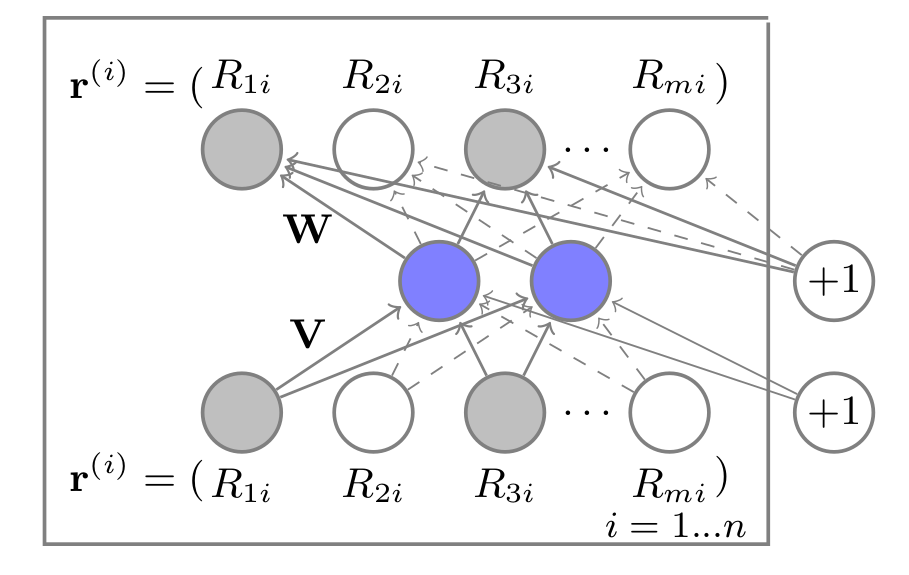
\includegraphics[scale=0.25]{autoenc.png}
\caption{Autoencoder for collaborative filtering \cite{autorec}}
\label{autoenc}
\end{figure} 
A random number set of observed ratings of $I_{i}$ will then be set to 0, corresponding to a non-observed rating. The objective function formalizes then a linear combination of the L2-error on the predicted output for these hidden values, and the L2-error on the output of the initially observed ratings.
As suggested in \cite{DBLP:journals/corr/StrubMG16}, the loss function will then be: 
$$
\begin{aligned}
L_{2,\alpha,\beta}(x,\widetilde{x}) = \alpha(\sum\limits_{j \in \mathcal{C}(\widetilde{x})} [nn(\widetilde{x})_{j}]^{2})+ \\ \beta(\sum\limits_{j \notin \mathcal{C}(\widetilde{x})} [nn(\widetilde{x})_{j}]^{2})
\end{aligned}
$$
where $\widetilde{x}$ is the corrupted version of $x$ and $nn(\widetilde{x}_j)$ is the $j^{th}$ of the network fed with $x$. 
\newline
Additionaly to adding L2-regularization terms for the network weights, we corrupt the input further as suggested in \cite{Vincent:2010:SDA:1756006.1953039}. Before hidding some part of the input, we first add random gaussian noise and what the authors call "salt and pepper" noise, which consists of randomly putting some elements to the minimum rating and some to the maximum rating.
\newline 
Finally, we also tested the possibility to add more layers to the autoencoder to learn more complex features as proposed in \cite{Kuchaiev2017TrainingDA}, but which didn't improve the predictions.

\end{description}

\subsection{Ensemble}

The performance of an invidual model can depend on multiple factors like the size of the rating matrix, its sparsity and other non-obvious parameters \cite{comparative}. 
To be able to combine the strength of each individual model, we determined the optimal linear combination of the predictions made by these models on a validation set. 
\[
\begin{bmatrix}
    pred_{1,1}  & \hdots & pred_{1,m}\\
    pred_{2,1}  & \hdots & pred_{2,m}\\
    \hdotsfor{3} \\
    pred_{d,1}  & \hdots & pred_{d,m}
\end{bmatrix}
\begin{bmatrix}
    w_{1}\\
    \hdots \\
    w_{m}\\
\end{bmatrix}
=
\begin{bmatrix}
    val_{1}\\
    val_{2}\\
    \hdotsfor{1} \\
    val_{d}
\end{bmatrix}
\]
where the d predictions of the m models are linearly combined. We also added a L2-regularization term to avoid overfitting on the validation set. 
\newline
We also tried to combine the features using a Multi Layer Perceptron, using the rows of the above left matrix as training input. Due to the complexity of this model, the variance had to be generously regularized. 
\newline
The results have been showing that it was essential to keep a small part of the training data exclusively for model combining so that the trained models can be combined over true validation data.  

\section{Evaluation}
\label{res}

\begin{table}[h!]
	\centering
	\begin{tabular}{l|l}
		\textit{\textbf{Model}} & \textit{\textbf{RMSE}} \\
		\hline
		SVD                     &       1.00468                 \\
		MF with SGD             &       1.02303                 \\
		\hline	
		k-means                 &        1.06                \\
		Item-Based              &        1.05                \\
		Ridge SVD               &        1.0264                \\
		AutoEncoder             &        0.99782               \\
		BPMF                    &        0.99355               \\
		RSVD       	            &        0.98787                \\
		NPCA                    &        0.98574                      
	\end{tabular}
\caption{Results of our models' evaluation}
\label{tabres}
\end{table}

\begin{table}[h!]
	\centering
	\begin{tabular}{l|l}
		\textit{\textbf{Ensemble}} & \textit{\textbf{RMSE}} \\
		\hline
		MLP                     &      0.97518                 \\
		Ridge      	            &         0.97331                                   
	\end{tabular}
\caption{Results of our ensemble methods' evaluation}
\label{ensres}
\end{table}

The results of the individual models are presented in \emph{Table \ref{tabres}}.
The two simple baseline models, which are both model-based matrix factorization models, both outperform the memory based models by at least 2.6\%. On the other hand, all the other improved matrix factorization methods except the regularized SGD, increase the RMSE by at least 1.11\%. By simply adding regularization to SVD with SGD, we outperformed all of our models except NPCA, which led to the best individual model score.
\\
The results of the ensemble on the individual models using MLP or Ridge Regression are presented in \emph{Table \ref{ensres}}. Both of them led to an improvement of at least 1.07\% compared to our best model, and Ridge regession showed to work best on our models and this dataset with an RMSE of 0.97331.

\section{Discussion}
\label{disc}

While it is not posible to fully assess the efficiency of the different methods when tested on a single dataset, there are still some relevant comments that can be made. 
As proposed in \cite{comparative}, matrix factorization based methods tend to be in general more accurate with increasing number of users. Our dataset consisting of 10000 users, this assumption is confirmed for our experiments, with a clear gap between memory-based and MF models. However, memory based methods are able to take in account specifities of the dataset that the matrix factorization methods aren't: if the predictions of the k-means algorithm and the item-based model are discarded for the Ridge Regression ensemble, the RMSE slightly increases from 0.97331 to 0.97350. On datasets where the memory-based methods are individually more accurate, we could expect this number to increase significantly more.\\
Despite the rise of machine learning based methods in many other research domains, the autoencoder hasn't shown as promising results as expected. In fact, when the AutoEncoder predictions are discarded when combining the models using Ridge Regression, the RMSE stays constant, which means that the AutoEncoder doesn't bring new insights comapred to the other models. Despite many tricks applied to the AutoEncoder such as adding different noise types and loss functions, the accuracy of the predictions is very dependent on the parameters and can thus quickly become less precise than expected. Also, as shown in \cite{Kuchaiev2017TrainingDA}, an autoencoder is nothing else than some matrix factorization, thanks to the few units on the hidden layer.\\
We have also shown that combining the models with a linear Ridge Regression significantly outperformed any of the individual models. Even if it is unclear at this state of the research how an individual model will perform on a given dataset \cite{comparative}, our results clearly show that each of them have strengths and limitations and that the strengths can easily be combined using the individual predictions. Finally, using an MLP to combine predicitions from 7 different sources didn't decrease the final RMSE. The model complexity led to overfitting on the validation set and thus the MLP ensemble prediction didn't score as well on the Kaggle test set.



\section{Conclusion}
\label{conc}

In this work we implemented and evaluated different Collaborative Filtering techniques to build reliable and efficient Recommender Systems. We first implemented 7 different individual models based on different papers and submitted their predictions to the Kaggle system to be able to compare their performances in terms of the Root Mean Squared Error, and analyse their strengths and limitations. To further improve the predictions, we implemented and tested two different types of ensemble models, the first using a Multi-Layer Perceptron and the second using Ridge Regression. Analysing both methods' predictions, we concluded that the latter was the best model in our situation. By using this approach, we were able to further enhance our results achieving a final score of 0.97331, corresponding to a final improvement of 4.972 \% compared to the best baseline and 1.26\% over our best individual model (NPCA).


\bibliographystyle{IEEEtran}
\bibliography{TeamName-literature}
\end{document}
